\documentclass[10pt, a4paper]{article}
\usepackage{preamble}

\newcommand{\mbf}[1]{\mathbf{#1}}

\title{Linear Algebra I}
\author{Luke Phillips}
\date{October 2024}

\begin{document}

\maketitle

\newpage

\section{Vectors and vector spaces}

\subsection{Vector space $\R ^ n$}

\begin{definition}
    $n$-dimensional real space $\R ^ n$ a set of elements as such\[
    \R ^ n = \left\{\underline{x} = \begin{pmatrix}
        x_1 \\
        x_2 \\
        \vdots \\
        x_n
    \end{pmatrix}
    \quad:\ x_i \in \R
    \right\}\footnote{Vectors are $\underline{x}$ or $\mbf{x}$.}\]
\end{definition}

\begin{definition}
    The zero vector is defined as
    \[
    \mbf{0} = \begin{pmatrix}
        0 \\
        0 \\
        \vdots \\
        0
    \end{pmatrix}
    \in \R ^ n
    \]
\end{definition}

There are two operations on $\R ^ n$

\textbf{Vector addition}:

Vector addition is a function defined as such
\[
\R ^ n \times \R ^ n \mapsto \R ^ n
\]
This function takes two vectors $\mbf{v, w}$ and obtains
\[
(\mbf{v, w})\mapsto \mbf{v + w}
\]
For example
\[
\mbf{v + w} = \begin{pmatrix}
    v_1 \\
    v_2 \\
    \vdots \\
    v_n
\end{pmatrix} + \begin{pmatrix}
    w_1 \\
    w_2 \\
    \vdots \\
    w_n
\end{pmatrix}
=
\begin{pmatrix}
    v_1 + w_1 \\
    v_2 + w_2 \\
    \vdots \\
    v_n + w_n
\end{pmatrix}
=
\mbf{v + w}
\]

\textbf{Scalar multiplication}:

Scalar multiplication is defined as a function
\[
\R \times \R ^ n \mapsto \R ^ n.
\]
This is written as follows
\[
(\lambda, \mbf{v}) \mapsto \lambda\mbf{v}
\]
The operation is defined as such
\[
\lambda\mbf{v} = \lambda\begin{pmatrix}
    v_1 \\
    v_2 \\
    \vdots \\
    v_n
\end{pmatrix}
=
\begin{pmatrix}
    \lambda v_1 \\
    \lambda v_2 \\
    \vdots \\
    \lambda v_n
\end{pmatrix}
\]

\textbf{Intuition}

Vectors can be thought of a point in $n$-dimensional space
\begin{figure}[h!]
    \centering
    \begin{tikzpicture}
    \draw[->] (0,0) -- (0,2);
    \draw[->] (0,0) -- (2,0);
    \draw[->] (0,0) -- (1.5,1);
    \filldraw (1,1) circle (2pt);
    \end{tikzpicture}
    \caption{Graph 1}
    \label{fig:Gr1}
\end{figure}

As a direction to a point
\begin{figure}[h!]
    \centering
    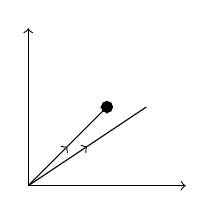
\begin{tikzpicture}
    \draw[->] (0,0) -- (0,2);
    \draw[->] (0,0) -- (2,0);
    \draw[->] (0,0) -- (0.75,0.5);
    \draw[-] (0.75,0.5) -- (1.5,1);
    \draw[->] (0,0) -- (0.5, 0.5);
    \draw[->] (0.5,0.5) -- (1, 1);
    \filldraw (1,1) circle (2pt);
    \end{tikzpicture}
    \caption{Graph 2}
    \label{fig:Gr2}
\end{figure}

As up to translation
\begin{figure}[h!]
    \centering
    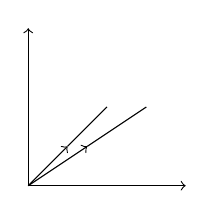
\begin{tikzpicture}
    \draw[->] (0,0) -- (0,2);
    \draw[->] (0,0) -- (2,0);
    \draw[->] (0,0) -- (0.75,0.5);
    \draw[-] (0.75,0.5) -- (1.5,1);
    \draw[->] (0,0) -- (0.5, 0.5);
    \draw[-] (0.5,0.5) -- (1, 1);
    \end{tikzpicture}
    \caption{Graph 3}
    \label{fig:Gr3}
\end{figure}

Vector addition
\begin{figure}[h!]
    \centering
    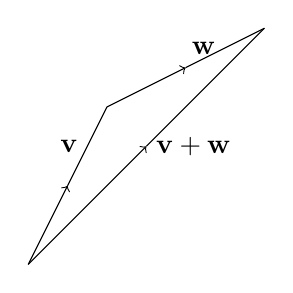
\begin{tikzpicture}
    \draw[->] (0,0) -- (0.5,1);
    \draw[-] (0.5,1) -- (1,2) node [midway, left] {$\mbf{v}$};
    \draw[->] (1,2) -- (2,2.5);
    \draw[-] (2,2.5) -- (3,3) node [midway, left] {$\mbf{w}$};
    \draw[->] (0,0) -- (1.5,1.5) node [right] {$\mbf{v + w}$};
    \draw[-] (1.5,1.5) -- (3,3);
    \end{tikzpicture}
    \caption{Graph 4}
    \label{fig:Gr4}
\end{figure}

Scalar multiplication
\begin{figure}[h!]
    \centering
    \begin{tikzpicture}
    \draw[->] (2,2) -- (3,3) node[left] {$\mbf{v}$};
    \draw[-] (3,3) -- (4,4);
    \draw[->] (2,0) -- (4,2) node[left] {$\mbf{\lambda v}$};
    \draw[->] (4,2) -- (6,4);
    \end{tikzpicture}
    \caption{Graph 5}
    \label{fig:Gr5}
\end{figure}
\textbf{Gr5}


These operations satisfy the \textbf{axioms} of a real vector space.
\begin{enumerate}[label = (\roman*)]
    \item There exists an additive identity $\mbf{0} \in \R ^ n$ such that
    \[
    \mbf{0 + v = v + 0 = v} \ \forall \mbf{v} \in \R ^ n.
    \]
    \item Commutativity
    \[
    \forall\mbf{w, v} \in \R ^ n\quad\mbf{w + v =  v + w}
    \]
    \item Existence of additive inverses
    \[
    \forall\mbf{v} \in \R ^ n\ \exists\mbf{-v} \in \R ^ n \text{ s.t. } \mbf{v + (-v) = (-v) + v = 0}
    \]
    \item Associativity
    $\forall\mbf{u, v, w} \in \R ^ n$
    \[
    (\mbf{u + v}) + \mbf{w} = \mbf{u} + (\mbf{v + w})
    \]
\end{enumerate}
(i), (iii), (iv) $\iff (\R ^ n, +)$ is a group

(i), (ii), (iii), (iv) $\iff (\R ^ n, +)$ is an abelian group \\


\textbf{Axioms} for scalar multiplication
\begin{enumerate}[label = (\roman*)]
    \item $0\mbf{v} = \mbf{0}\quad\forall\mbf{v}\in \R ^ n$.
    \item $1\mbf{v} = \mbf{v}\quad\forall\mbf{v}\in \R ^ n$.
    \item Associativity
    \[
    \lambda (\mu\mbf{v}) = (\lambda\mu)\mbf{v}\quad\forall\lambda,\mu \in \R\quad\forall\mbf{v}\in\R ^ n
    \]
    \item Distributivity, $\forall\lambda,\mu\in\R\quad\forall\mbf{v, w} \in \R ^ n$
    \begin{align*}
    (\lambda + \mu)\mbf{v} &= \lambda\mbf{v} + \mu\mbf{v} \\
    \lambda(\mbf{v + w}) &= \lambda\mbf{v} + \lambda\mbf{w}
    \end{align*}
\end{enumerate}

$\R ^ n$ clearly satisfies these axioms (if not obvious check) because they can be checked component-wise once we set 
\[
-\mbf{v} = \begin{pmatrix}
    -v_1 \\
    -v_2 \\
    \vdots \\
    -v_n
\end{pmatrix}
\]

\begin{definition}
    Standard basis vectors
    
    For $1 \leq i \leq n$ we define $\mbf{e}_i \in \R ^ n$
    \[
    \mbf{e}_i = \begin{pmatrix}
        0 \\
        0 \\
        \vdots \\
        0 \\
        1\footnote{$i$th position from the top.} \\
        0 \\
        \vdots \\
        0
    \end{pmatrix}
    \]    
\end{definition}

\begin{example}
    \[
    \mbf{e}_1 = \begin{pmatrix}
        1 \\
        0 \\
        \vdots \\
        0
    \end{pmatrix}
    \]
    \[
    \mbf{e}_2 = \begin{pmatrix}
        0 \\
        1 \\
        \vdots \\
        0
    \end{pmatrix}
    \]
\end{example}

We can express any vector $\mbf{x} \in \R ^ n$ uniquely as a linear combination of the standard basis vectors.

\begin{example}
    \begin{align*}
    \mbf{x} &= \begin{pmatrix}
        x_1 \\
        x_2 \\
        \vdots \\
        x_n
    \end{pmatrix}
    =
    x_1 \begin{pmatrix}
        1 \\
        0 \\
        \vdots \\
        0
    \end{pmatrix}
    +
    x_2 \begin{pmatrix}
        0 \\
        1 \\
        \vdots \\
        0
    \end{pmatrix}
    +
    \dots
    +
    x_n \begin{pmatrix}
        0 \\
        0 \\
        \vdots \\
        0 \\
        1
    \end{pmatrix} \\
    &= x_1 \mbf{e}_1 + x_2 \mbf{e}_2 + \dots + x_n \mbf{e}_n
    \end{align*}
\end{example}
The $x_i$'s are sometimes called the Cartesian coordinates of the vector $\mbf{x}$.

\subsection{The scalar (or dot) product in $\R ^ n$}

\begin{definition}
    The scalar product is defined as $\R ^ n \times \R ^ n \mapsto \R$, $(\mbf{u, v}) \mapsto \mbf{u \cdot v}$
    \begin{align*}
    \mbf{u \cdot v} &= \begin{pmatrix}
        u_1 \\
        u_2 \\
        \vdots \\
        u_n
    \end{pmatrix} \cdot
    \begin{pmatrix}
        v_1 \\
        v_2 \\
        \vdots \\
        v_n
    \end{pmatrix} \\
    &= u_1 v_1 + u_2 v_2 + \dots + u_n v_n  \\
    &= \sum_{i = 1}^{n}u_iv_i \in \R
    \end{align*}
\end{definition}

\begin{example}
    \[
    \begin{pmatrix}
        4 \\
        1 \\
        2
    \end{pmatrix}
    \cdot
    \begin{pmatrix}
        -3 \\
        -2 \\
        1
    \end{pmatrix}
    =
    -12 - 2 + 2 = -12.
    \]
\end{example}


\textbf{Axioms} of the scalar product
% To-Do add in the foralls here
\begin{enumerate}[label = (\roman*)]
    \item Symmetry
    \[
    \mbf{u \cdot v = v \cdot u}\qquad\forall\mbf{u, v} \in \R ^ n
    \]
    \item Linearity (1)
    \begin{align*}
    (\mbf{u + v)\cdot w}) &= \mbf{u \cdot w + v \cdot w}\qquad\forall \lambda \in \R\\
    \lambda\mbf{u})\cdot \mbf{w} &= \lambda (\mbf{u \cdot w})\qquad\forall\mbf{u, v, w} \in \R ^ n
    \end{align*}
    \item Linearity (2)
    \begin{align*}
        \mbf{u} \cdot (\mbf{v + w}) &= \mbf{u} \cdot \mbf{v} + \mbf{u} \cdot \mbf{w}\qquad \forall \lambda \in \R \\
        \mbf{u} \cdot \lambda\mbf{v} &= \lambda(\mbf{u \cdot v})\qquad \forall\mbf{u, v, w} \in \R ^ n
    \end{align*}
    \item Positivity
    \begin{align*}
        \mbf{v \cdot v} \geq 0\quad \forall \mbf{v} \in \R ^ n \\
        \text{and } \mbf{v \cdot v} = 0 \iff \mbf{v = 0}
    \end{align*}
\end{enumerate}

\begin{definition}
    Given a vector $\mbf{v} \in \R ^ n$ we define its magnitude (or length) to be
    \[
    |\mbf{v}| = \sqrt{\mbf{v \cdot v}}
    \]
\end{definition}
Note $\mbf{v \cdot v} \geq 0$ so positive square roots exist. Likewise note

$|\mbf{v}| \geq 0 \text{ and } |\mbf{v}| = 0 \iff \mbf{v = 0}$

\begin{example}
    \[
    \left|\begin{pmatrix}
        -3 \\
        4
    \end{pmatrix}\right|
    = \sqrt{(-3) ^ 2 + 4 ^ 2} = \sqrt{25} = 5
    \]
\end{example}

Thinking about a vector $\mbf{v} \in \R ^ 2$ where $\mbf{v \neq 0}$
\begin{figure}[h!]
    \centering
    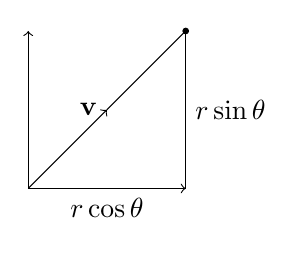
\begin{tikzpicture}
    \draw[->] (0,0) -- (0,2);
    \draw[->] (0,0) -- (2,0);
    \draw[->] (0,0) -- (1,1) node[left] {$\mbf{v}$};
    \draw[-] (1,1) -- (2,2);
    \draw[-] (2,0) -- (2,2) node[midway, right] {$r\sin\theta$};
    \draw[-] (0,0) -- (2,0) node[midway, below] {$r\cos\theta$};
    \filldraw (2,2) circle (1pt);
    \end{tikzpicture}
    \caption{Graph 9}
    \label{fig:Gr9}
\end{figure}

\[
\mbf{v}  = \begin{pmatrix}
    r\cos\theta \\
    r\sin\theta
\end{pmatrix}
\]
where
$r = |\mbf{v}|$ and $0 \leq \theta < 2\pi$, $\theta$ is the angle made by $\mbf{v}$ in an anticlockwise direction with the positive real axis.

We define $(r, \theta) \in (0, \infty) \times [0, 2\pi)$
to be the unique numbers such that
$\mbf{v}  = \begin{pmatrix}
    r\cos\theta \\
    r\sin\theta
\end{pmatrix}$
we call $(r, \theta)$ the polar coordinates of $\mbf{v}$

\begin{example}
    Suppose $\mbf{v} = \begin{pmatrix}
        2 \\
        3
    \end{pmatrix}$,
    what are its polar coordinates?

    $r = |\mbf{v}| = \sqrt{2 ^ 2 + 3 ^ 2} = \sqrt{13}$

    $\theta = \arcsin \left({\dfrac{3}{\sqrt{13}}}\right)$
\end{example}

\begin{example}
    Suppose $\mbf{v} = \begin{pmatrix}
        2 \\
        -2
    \end{pmatrix}$,
    what are its polar coordinates?

    $r = |\mbf{v}| = \sqrt{2 ^ 2 + (-2) ^ 2} = \sqrt{8} = 2\sqrt{2}$

    $\theta = \dfrac{7\pi}{4}$
\end{example}

\begin{proposition}
    Suppose $\mbf{v}, \mbf{w} \in \R ^ n$
    \[
    |\mbf{v}| = r,\quad|\mbf{w}| = s
    \]
    Suppose that $\mbf{v}, \mbf{w}$ make an angle of $\alpha$ with each other $0 \leq \alpha \leq \pi$
    
    Then $\mbf{v}\cdot\mbf{w} = rs\cos(\alpha)$.
    \begin{proof}
        Suppose polar coordinated of $\mbf{v}$ are $(r, \theta)$, and of $\mbf{w}$ are $(s, \varphi)$.

        Then $\mbf{v} = \begin{pmatrix}
            r\cos\theta \\
            r\sin\theta
        \end{pmatrix}$, $\mbf{w} = \begin{pmatrix}
            s\cos\varphi \\
            s\sin\varphi
        \end{pmatrix}$
        \begin{align*}
        \mbf{v\cdot w} &= \begin{pmatrix}
            r\cos\theta \\
            r\sin\theta
        \end{pmatrix} \cdot \begin{pmatrix}
            s\cos\varphi \\
            s\sin\varphi
        \end{pmatrix} \\
        &= rs\cos\theta\cos\varphi + rs\sin\theta\sin\varphi \\
        &= rs(\cos\theta\cos\varphi + \sin\theta\sin\varphi) \\
        &= rs(\cos(\theta - \varphi) \\
        &= rs\cos(\pm\alpha) = rs\cos\alpha.
        \end{align*}
    \end{proof}
\end{proposition}

\begin{corollary}
    If $\mbf{v} \neq \mbf{0}$ and $\mbf{w} \neq \mbf{0}$.
    $\mbf{v}$ and $\mbf{w}$ are orthogonal if and only if
    \[
    \mbf{v \cdot w} = 0.
    \]
    \begin{proof}
        \[
        \mbf{v \cdot w} = 0 \iff \cos(\alpha) = 0 \iff \alpha = \frac{\pi}{2}
        \]
    \end{proof}
\end{corollary}

\begin{example}
    $\mbf{v} = \begin{pmatrix}
        6 \\
        -2
    \end{pmatrix}\qquad
    \mbf{w} = \begin{pmatrix}
        -1 \\
        -3
    \end{pmatrix}$

    Then $\mbf{v\cdot w} = 6(-1) + (-2)(-3) = 0$

    So $\mbf{v, w}$ are orthogonal.
\end{example}


\begin{theorem}[Cauchy-Schwarz inequality]
    Suppose $\mbf{u, v} \in \R ^ n$, $\mbf{u, v} \neq 0$ then we have
    \[
    |\mbf{u}||\mbf{v}| \geq |\mbf{u \cdot v}|
    \]
    with equality if and only if $\mbf{u, v}$ are parallel (multiples of each other).
\end{theorem}

\begin{definition}
    Suppose $\mbf{u, v} \in \R ^ n$ with $\mbf{u, v \neq 0}$ then we define the angle between them to be the unique $0 \leq \theta \leq \pi$ such that $\mbf{u \cdot v} = |\mbf{u}||\mbf{v}|\cos\theta$.
\end{definition}

\begin{example}
    Find the angle between the vectors 
    \[
    \mbf{v} = \begin{pmatrix}
        1 \\ 2 \\ 1 \\ 3
    \end{pmatrix}, \quad \mbf{w} = \begin{pmatrix}
        1 \\ 3 \\ -1 \\ 3
    \end{pmatrix} \in \R ^ 4.
    \]
    Find $\theta$ s.t. $\mbf{v\cdot w} = |\mbf{v}||\mbf{w}|\cos\theta$

    $|\mbf{v}| = \sqrt{1 ^ 2 + 2 ^ 2 + 1 ^ 2 + 3 ^ 2} = \sqrt{1 + 4 + 1 + 9} = \sqrt{15}$
    
    $|\mbf{w}| = \sqrt{1 ^ 2 + 3 ^ 2 + (-1) ^ 2 + 3 ^ 2} = \sqrt{1 + 9 + 1 + 9} = \sqrt{20} = 2\sqrt{5}$

    $\mbf{v \cdot w} = 1 + 6 + -1 + 9 = 15$
    \[
    \cos\theta = \frac{\mbf{v \cdot w}}{|\mbf{v}||\mbf{w}|} = \frac{15}{\sqrt{15}\sqrt{20}} = \frac{\sqrt{15}}{\sqrt{20}} = \frac{\sqrt{3}}{\sqrt{4}} = \frac{\sqrt{3}}{2}
    \]
    $\theta = \dfrac{\pi}{6}$.
\end{example}

For $\mbf{v, w} \in \R ^ n$ $\mbf{v, w \neq 0}$ if $\mbf{v \cdot w} = 0$ (so they make an angle of $\frac{\pi}{2}$) we call $\mbf{v, w}$ orthogonal.

\begin{example}
    Find all unit\footnote{$|\mbf{w}| = 1$} vectors $\mbf{w} \in \R ^ 3$ that make an angle of $\frac{\pi}{4}$ with both.
    \[
    \mbf{u} = \begin{pmatrix} 1 \\ -1 \\ 0 \end{pmatrix},
    \quad\mbf{v} = \begin{pmatrix} 1 \\ 0 \\ 1 \end{pmatrix}.
    \]

    Suppose $\mbf{w} = \begin{pmatrix} w_1 \\ w_2 \\ w_3 \end{pmatrix}$ is a solution.

    First note $|\mbf{u}| = \sqrt{1 ^ 2 + (-1) ^ 2} = \sqrt{2}$,\quad$|\mbf{v}| = \sqrt{1 ^ 2 + 1 ^ 2} = \sqrt{2}$
    Now $\mbf{u \cdot w} = |\mbf{u}||\mbf{w}|\cos\left(\frac{\pi}{4}\right) = \sqrt{2} \cdot 1 \cdot \frac{1}{\sqrt{2}} = 1$

    and $\mbf{v \cdot w} = |\mbf{v}||\mbf{w}|\cos\left(\frac{\pi}{4}\right) = \sqrt{2} \cdot 1 \cdot \frac{1}{\sqrt{2}} = 1$.

    So $w_1 - w_2 = 1$ and $w_1 + w_3 = 1$. So $w_2 = w_1 - 1$ and $w_3 = 1 - w_1$.
    Also $\mbf{w \cdot w} = 1$ so $w_1 ^ 2 + w_2 ^ 2 + w_3 ^ 2 = 1$.
    Hence $w_1 ^ 2 + (w_1 - 1) ^ 2 + (1 - w_1) ^ 2 = 1$
    solve for $w_1$ (two solutions)
\end{example}

\subsection{The vector product}
The vector product (or cross product)
\[
\R ^ 3 \times \R ^ 3 \rightarrow \R ^ 3
\]
\[
(\mbf{u, v}) \mapsto \mbf{u \times v}
\]

\begin{definition}
    \[
    \mbf{x \times y} = \begin{pmatrix}
        x_1 \\ x_2 \\ x_3
    \end{pmatrix}
    \times
    \begin{pmatrix}
        y_1 \\ y_2 \\ y_3
    \end{pmatrix}
    =
    \begin{pmatrix}
        x_2 y_3 - x_3 y_2 \\
        x_3 y_1 - x_1 y_3 \\
        x_1 y_2 - x_2 y_1
    \end{pmatrix}
    \]
\end{definition}

\begin{example}
    \[
    \begin{pmatrix}
        7 \\ -4 \\ 2   
    \end{pmatrix}
    \times
    \begin{pmatrix}
        2 \\ 3 \\ -1
    \end{pmatrix}
    =
    \begin{pmatrix}
        (-4)(-1) - 2 \cdot 3 \\
        2 \cdot 2 - 7 \cdot (-1) \\
        7 \cdot 3 - (-4)(2)
    \end{pmatrix}
    =
    \begin{pmatrix}
        -2 \\ 11 \\ 29
    \end{pmatrix}
    \]
\end{example}

Properties of the cross product
\begin{enumerate}[label = (\roman*)]
    \item Anti-symmetry: $\mbf{u \times v} = -(\mbf{v \times u})$\quad$\forall\mbf{u, v} \in \R ^ 3$
    \item Linearity 1:
    $(\mbf{u + v} \times \mbf{w} = \mbf{u \times w} + \mbf{v \times w}$\quad$\forall\lambda \in \R$
    
    $(\lambda\mbf{u}) \times \mbf{v} = \lambda(\mbf{u \times v})$\quad$\forall\mbf{u, v, w} \in \R ^ 3$
    
    \item Linearity 2:
    $\mbf{u} \times (\mbf{v + w}) = \mbf{u \times v + u \times w}$\quad$\forall\lambda \in \R$
    
    $\mbf{u} \times (\lambda\mbf{v}) = \lambda\mbf{u \times w}$\quad$\forall\mbf{u, v, w} \in \R ^ 3$

    \item Orthogonality to the input
    \[
    \mbf{u \cdot (u \times v)} = 0 = \mbf{v \cdot (u \times v)}\quad\forall\mbf{u, v} \in \R ^ 3
    \]
\end{enumerate}
In other words $\mbf{u \times v}$ is orthogonal to $\mbf{u}$ and $\mbf{v}$.

\begin{lemma}
    Suppose that $\mbf{x, y} \in \R ^ 3$ are vectors of length $|\mbf{x}| = r > 0$, $|\mbf{y}| = s > 0$. Then
    \[
    |\mbf{x \times y}| = rs\sin\theta
    \]
    where $0 \leq \theta \leq \pi$ is the angle between $\mbf{x}$ and $\mbf{y}$.
    
    \begin{proof}
        \begin{align*}
            |\mbf{x\times y}| ^ 2 &= (\mbf{x} \times \mbf{y}) \cdot (\mbf{x} \times \mbf{y}) \\
            &= (x_2y_3 - x_3y_2) ^ 2 + (x_3y_1 - x_1y_3) ^ 2 + (x_1y_2 - x_2y_1) ^ 2 \\
            &= (x_1 ^ 2 + x_2 ^ 2 + x_3 ^ 2)(y_1 ^ 2 + y_2 ^ 2 + y_3 ^ 2) - (x_1y_1 + x_2y_2 + x_3y_3) ^ 2 \\
            &= r ^ 2 s ^ 2 - (\mbf{x \cdot y}) ^ 2 \\
            &= r ^ 2 s ^ 2 - r ^ 2 s ^ 2 \cos ^ 2\theta \\ 
            &= r ^ 2 s ^ 2 (1 - \cos ^ 2\theta) \\ 
            &= r ^ 2 s ^ 2 \sin ^ 2 \theta 
        \end{align*}
    \end{proof}
\end{lemma}

\begin{example}
    \[
    \left|\begin{pmatrix}
        7 \\ -4 \\ 2   
    \end{pmatrix}\right| = \sqrt{49 + 16 + 4} = \sqrt{69}
    \]
    \[
    \left|\begin{pmatrix}
        2 \\ 3 \\ -1
    \end{pmatrix}\right| = \sqrt{4 + 9 + 1} = \sqrt{14}
    \]
    \[
    \left|\begin{pmatrix}
        7 \\ -4 \\ 2   
    \end{pmatrix}
    \times
    \begin{pmatrix}
        2 \\ 3 \\ -1
    \end{pmatrix}\right| = \left|\begin{pmatrix}
        -2 \\ 11 \\ 29
    \end{pmatrix}\right| = \sqrt{4 + 121 + 861} = \sqrt{966}.
    \]
    If $\theta$ is the angle between $\begin{pmatrix}
        7 \\ -4 \\ 2   
    \end{pmatrix}$ and $\begin{pmatrix}
        2 \\ 3 \\ -1
    \end{pmatrix}$ we have $\sqrt{966} = \sqrt{69}\sqrt{14}\sin\theta$ so $\sin\theta = 1$ and $\theta = \frac{\pi}{2}$.
\end{example}

\subsection{Planes in $\R ^ 3$}

\textbf{The parametric form}

Let $\Pi \subseteq \R ^ 3$ be a plane. $\mbf{a} \in \Pi$, point on the plane $\Pi$. $\mbf{d}_1, \mbf{d}_2 \in \R ^ 3$ parallel to $\Pi$ but not parallel to each other (i.e. "collinear"). $\mbf{d}_1 \neq 0$, $\mbf{d}_2 \neq 0$.

To get to any point $\mbf{p} \in \Pi$, first travel to the point $\mbf{a} \in \Pi$ then along $\mbf{d}_1$ and $\mbf{d}_2$ some amount. So
\[
\Pi = \{\mbf{a} + \lambda_1\mbf{d}_1 + \lambda_2\mbf{d}_2\,|\,\lambda_1, \lambda_2 \in \R\}.
\]
$\lambda_1, \lambda_2$ are called "free variables"\footnote{Or "free parameters".}. \\

\textbf{Using the normal vector}

Let $\Pi \subseteq \R ^ 3$ be a plane. $\mbf{a} \in \Pi$, $\mbf{n}$ is a normal vector to $\Pi$, ($n \neq 0$), 
\begin{align*}
    \mbf{x} \in \Pi &\iff (\mbf{x - a}) \text{ is orthogonal to } \mbf{n} \\
    &\iff (\mbf{x - a}) \cdot \mbf{n} = 0 \\
    &\iff \mbf{x \cdot a} - \mbf{a \cdot n} = 0 \\ 
    &\iff \mbf{x \cdot a} = \mbf{a \cdot n} \\ 
    &\iff \mbf{x \cdot a} = \ell.
\end{align*}

\begin{align*}
    \Pi &= \{\mbf{x} \in \R ^ 3\,|\,\mbf{x\cdot a} = \mbf{a \cdot n}\} \\
    &= \{\mbf{x} \in \R ^ 3\,|\, \mbf{x \cdot n} = \ell\}.
\end{align*}

\textbf{Cartesian form}

((B) in coordinates)

If we write $\mbf{n} = \begin{pmatrix}
    a \\ b \\ c
\end{pmatrix},\ \mbf{x} = \begin{pmatrix}
    x \\ y \\ z
\end{pmatrix}$ then $\mbf{n \cdot x} = \ell$ can be written:
\[
ax + by + cz = \ell
\]
So
\[
\Pi = \left\{\begin{pmatrix}
    x \\ y \\ z
\end{pmatrix} \in \R ^ 3\,|\, ax + by + cz = \ell\right\}.
\]

\begin{example}
    Find the Cartesian description of the plane $\Pi$ that passes through $\begin{pmatrix}
        1 \\ -1 \\ 3
    \end{pmatrix}$ and is normal to the direction $\begin{pmatrix}
        5 \\ 2 \\ 1
    \end{pmatrix}$.

    $\mbf{n} = \begin{pmatrix}
        5 \\ 2 \\ 1
    \end{pmatrix},\, \mbf{a} = \begin{pmatrix}
        1 \\ -1 \\ 3
    \end{pmatrix} \in \Pi$.
    \begin{align*}
    \Pi &= \left\{ \begin{pmatrix}
        x \\ y \\ z
    \end{pmatrix} \in \R ^ 3\,|\, \mbf{x \cdot n = a \cdot n}\right\} \\
    &=\left\{\begin{pmatrix}
        x \\ y \\ z
    \end{pmatrix} \in \R ^ 3\,|\, 5x + 2y + z = 6\right\}
    \end{align*}
\end{example}

\begin{example}
    Find a normal vector to and a point on the plane
    \[
    6x - 5y + 3z = 30
    \]
    $\mbf{n} = \begin{pmatrix}
        6 \\ -5 \\ 3
    \end{pmatrix}$, $\mbf{a}$ can be any point on the plane e.g. $\begin{pmatrix}
        5 \\ 0 \\ 0
    \end{pmatrix},\,\begin{pmatrix}
        0 \\ -6 \\ 0
    \end{pmatrix} \text{ or } \begin{pmatrix}
        0 \\ 0 \\ 10
    \end{pmatrix}$
\end{example}

Parametric description from normal/Cartesian.

Suppose 
\begin{align*}
    \Pi &= \{\mbf{x} \in \R ^ 3 \,|\, \mbf{n\cdot x} = \ell\}
    &= \left\{\begin{pmatrix} x \\ y \\ z
    \end{pmatrix} \in \R ^ 3 \,|\, ax + by + cz = \ell\right\}
\end{align*}
where $\mbf{n} = \begin{pmatrix} a \\ b \\ c \end{pmatrix}$

If $c \neq 0$ then \[
ax + by + cz = \ell \iff z = \frac{\ell}{c} - \left(\frac{a}{c}\right)x - \left(\frac{b}{c}\right)y.
\]
So
\[
\Pi = \left\{ \begin{pmatrix}
    0 \\ 0 \\ \frac{\ell}{c}
\end{pmatrix} + x\begin{pmatrix}
    1 \\ 0 \\ -\frac{a}{c} 
\end{pmatrix} + y\begin{pmatrix}
    0 \\ 1 \\ -\frac{b}{c}
\end{pmatrix}\,:\, x, y \in \R \right\}
\]
(where $x, y$ are "free parameters")

Likewise similarly if $a \neq 0$ or $b \neq 0$ (cannot have $a = b = c = 0$)

\begin{example}
    Find parametric and Cartesian description of the plane $\Pi \subseteq \R ^ 3$ that passes through
    \[
    \mbf{a} = \begin{pmatrix}
        1 \\ 0 \\ 1
    \end{pmatrix}
    \quad
    \mbf{b} = \begin{pmatrix}
        2 \\ -1 \\ 3
    \end{pmatrix},
    \quad
    \mbf{c} = \begin{pmatrix}
        5 \\ 1 \\ 1
    \end{pmatrix}.
    \]

    Set $\mbf{d}_1 = \mbf{b - a} = \begin{pmatrix}
        1 \\ -1 \\ 2
    \end{pmatrix}$, $\mbf{d}_2 = \mbf{c - a} = \begin{pmatrix}
        4 \\ 1 \\ 0
    \end{pmatrix}$

    So $\Pi = \{\mbf{a} + \lambda_1 \mbf{d}_1 + \lambda_2 \mbf{d}_2\,|\, \lambda_1, \lambda_2 \in \R\}$

    $\mbf{n} = \mbf{d}_1 \times \mbf{d}_2$ then $\mbf{n}$ is normal to $\mbf{d}_1$ and $\mbf{d}_2$ and so is normal to $\Pi$.
    \[
    \mbf{n} = \begin{pmatrix}
        1 \\ -1 \\ 2
    \end{pmatrix}
    \times \begin{pmatrix}
        4 \\ 1 \\ 0
    \end{pmatrix}
    =
    \begin{pmatrix}
        -2 \\ 8 \\ 5
    \end{pmatrix}
    \]
    $\ell = \mbf{n \cdot a} = -2 + 5 = 3$.

    So we have
    \[
    \Pi = \left\{\begin{pmatrix}
        x \\ y \\ z
    \end{pmatrix} \in \R ^ 3\,|\, -2x + 8y + 5z = 3\right\}
    \]
\end{example}

\subsection{Lines}

\textbf{Parametric}

$L \subseteq \R ^ 3$. Take $\mbf{a} \in L$, $\mbf{d} \neq 0$ parallel to $L$. Then
\[
L = \{\mbf{a} +\lambda\mbf{d}\,|\, \lambda \in \R\}
\]

\textbf{Cartesian}

Set $\mbf{a} = \begin{pmatrix}
    a_1 \\ a_2 \\ a_3
\end{pmatrix},\quad\mbf{d} = \begin{pmatrix}
    d_1 \\ d_2 \\ d_3
\end{pmatrix}$


\[
\begin{pmatrix}
    x \\ y \\ z
\end{pmatrix} \in L \iff
\]
\begin{align*}
    a_1 + \lambda d_1 &= x \\
    a_2 + \lambda d_2 &= y \\
    a_3 + \lambda d_3 &= z
\end{align*}
for some $\lambda \in \R$

Suppose $d_1 \neq 0,\, d_2 \neq 0,\,d_3 \neq 0$ then
\[
\lambda = \frac{x - a_1}{d_1},\,\lambda = \frac{y - a_2}{d_2},\,\lambda = \frac{z - a_3}{d_3}.
\]

So
\[
\begin{pmatrix}
    x \\ y \\ z
\end{pmatrix} \in L \iff
\frac{x - a_1}{d_1} = \frac{y - a_2}{d_2} = \frac{z - a_3}{d_3}.
\]

So 
\[
L = \left\{\begin{pmatrix}
    x \\ y \\ z
\end{pmatrix} \in \R ^ 3 | \frac{x - a_1}{d_1} = \frac{y - a_2}{d_2} = \frac{z - a_3}{d_3}\right\}.
\]

If $d_1, d_2 \neq 0,\,d_3 = 0$ then $\lambda = \frac{x - a_1}{d_1} = \frac{y - a_2}{d_2},\, z = a_3$.

If $d_1 \neq 0,\,d_2 = d_3 = 0$ then $y = a_2,\, z = a_3$.


\textbf{Intersection of two planes}

Suppose $\Pi_i = \{\mbf{x} \in \R ^ 3 \,|\, n_i \cdot \mbf{x} = \ell_i\}$ for $i = 1, 2$. Then, what is
\[
Pi_1 \cap \Pi_2 = \{\mbf{x}\in \R ^ 3 \,|\, \mbf{n}_1 \cdot \mbf{x} = \ell_1,\,\mbf{n}_2 \cdot \mbf{x} = \ell_2\}.
\]

If $\mbf{n}_1$ and $\mbf{n}_2$ are parallel (collinear) then either $\Pi_1 = \Pi_2$ or if $\Pi_1 \neq \Pi_2$ then $\Pi_1 \cap \Pi_2 = \emptyset$.

If $\mbf{n}_1$ and $\mbf{n}_2$ are not parallel then $\Pi_1 \cap \Pi_2 = L$ for some line $L$

So 
\[L = \{\mbf{x}\in \R ^ 3 \,|\, \mbf{n}_1 \cdot \mbf{x} = \ell_1,\,\mbf{n}_2 \cdot \mbf{x} = \ell_2\} = \left\{\begin{pmatrix}
    x \\ y \\ z
\end{pmatrix} \in \R ^ 3 |
    ax + by + cz = \ell_1,
    dx + ey + fz = \ell_2
\right\}
\]

Given a description of $L$ as in the intersection of two planes, how do we get the parametric description of $L$?
We need $\mbf{a} \in L,\,\mbf{d \neq 0}$ where $\mbf{d}$ is parallel to $L$.

$\mbf{d}$ is parallel to $\Pi_1$ and $\Pi_2$ so $\mbf{d} \cdot \mbf{n}_1 = 0$, and $\mbf{d} \cdot \mbf{n}_2 = 0$ so set $\mbf{d} = \mbf{n}_1 \times \mbf{n}_2 = \begin{pmatrix}
    a \\ b \\ c
\end{pmatrix} \times \begin{pmatrix}
    d \\ e \\ f
\end{pmatrix} = \begin{pmatrix}
    bf - ce \\
    cd - af \\
    ae - bd
\end{pmatrix}$.

To find $\mbf{a} \in L$

If $ae - bd \neq 0$ then

$\mbf{d}$ has some "$z$-component",

so $L$ intersects the $(x, y)$-plane at a unique point $\mbf{a} = \begin{pmatrix}
    g \\ h \\ 0
\end{pmatrix}$

$g, h$ satisfy
\begin{align*}
    ag + bh + 0 &= \ell_1 \\
    dg + eh + 0 &= \ell_2
\end{align*}
Solve for $g, h$.


\end{document}